\documentclass{beamer}
\usetheme{Madrid} % A common, clean theme
\usecolortheme{default}

% \usepackage[utf8]{inputenc} % Removed, not needed with lualatex/xelatex
\usepackage[T1]{fontenc}
\usepackage{lmodern}
\usepackage[english]{babel}
\usepackage{amsmath, amssymb, mathtools}
\usepackage{graphicx}
\usepackage{xcolor}
\usepackage{hyperref}
\usepackage{xurl} % For better URL line breaking
\usepackage{booktabs} % For tables
\usepackage{siunitx}  % For number formatting in tables

% Title Info
\title{StyCLIP: StyleTransfer in Few-Shot Learning}
\author{Emanuele Fontana}
\institute{Università degli Studi di Bari Aldo Moro \\ \nolinkurl{e.fontana7@studenti.uniba.it}} % \nolinkurl and manual break if needed

% Define some commands from the original paper if needed for consistency
\newcommand{\Ft}{\mathbf{F}_\text{t}}      % Text features
\newcommand{\Fv}{\mathbf{F}_\text{v}}      % Visual features (support)
\newcommand{\Wt}{\mathbf{W}_\text{t}}      % Text prototypes
\newcommand{\Wv}{\mathbf{W}_\text{v}}      % Visual prototypes (support)
\newcommand{\fv}{\mathbf{f}_\text{v}}      % Query visual feature
\newcommand{\Figt}{\mathbf{F}_\text{IGT}}  % IGT features
\newcommand{\Ftgi}{\mathbf{F}_\text{TGI}}  % TGI features
\newcommand{\R}{\mathbb{R}}

\begin{document}
% --- Title Slide ---
\begin{frame}
  \titlepage
\end{frame}


% --- Introduction ---
\section{Introduction}
\begin{frame}
  \frametitle{Introduction \& Motivation}
  \begin{itemize}
    \item \textbf{Challenge:} Visual artist classification is crucial for art history and content analysis, especially with growing digital collections.
    \item \textbf{Focus:} Few-shot learning (FSL) for artist classification -- identifying artists with limited labeled examples.
    \item \textbf{Problem:}
      \begin{itemize}
        \item Artistic style involves subtle visual cues (brushstrokes, color palettes, composition).
        \item CLIP-based FSL methods excel at semantics but might overlook fine-grained stylistic nuances.
      \end{itemize}
    \item \textbf{Hypothesis:} Integrating explicit style representations (Gram matrices) into CLIP could enhance artist-specific pattern capture.
    \item \textbf{Proposal:} StyCLIP, a CLIP extension incorporating style features.
  \end{itemize}
\end{frame}

% --- Related Work ---
\section{Related Work}
\begin{frame}
  \frametitle{Related Work}
  \begin{block}{Style Transfer}
    \begin{itemize}
        \item Gatys et al. \cite{StyleTransfer}: Deep networks encode style in intermediate layers; Gram matrices capture style.
    \end{itemize}
  \end{block}

  \begin{block}{Few-Shot Learning (FSL) \& Meta-Learning}
    \begin{itemize}
        \item Prototypical Networks \cite{ProtoNet}: Learn to learn from small samples.
    \end{itemize}
  \end{block}

  \begin{block}{Contrastive Language-Image Pretraining (CLIP)}
    \begin{itemize}
        \item CLIP \cite{CLIP}: Shared embedding space for images and text.
        \item TIP-Adapter \cite{TipAdapter}: Non-parametric cache model for FSL.
        \item APE \cite{APE}: Adaptive prior refinement of CLIP features.
        \item GDA-CLIP \cite{GDA_CLIP}: Gradient-based adaptation.
        \item TIMO \cite{TIMO}: Mutual guidance between text/image modalities.
    \end{itemize}
  \end{block}
  \tiny
  \bibliographystyle{plain} % Use a simple style for beamer
  \nocite{StyleTransfer,ProtoNet,CLIP,TipAdapter,APE,GDA_CLIP,TIMO} % Cite them so they appear
\end{frame}

% --- Dataset ---
\section{Dataset}
\begin{frame}
  \frametitle{Dataset: ArtGraph Subset}
  \begin{itemize}
    \item Derived from ArtGraph dataset \cite{ArtGraph} (>100,000 paintings).
    \item Two non-overlapping subsets created:
  \end{itemize}
  \begin{columns}[T]
    \begin{column}{0.5\textwidth}
      \begin{block}{ArtGraph Few-Shot Subset (Evaluation)}
        \begin{itemize}
          \item \textbf{Style Selection:} Top 10 styles by artwork count.
          \item \textbf{Artist Filtering:} 30--50 artworks/style (up to 10 artists/style).
          \item \textbf{Splits:} 80\% support, 10\% validation, 10\% query.
        \end{itemize}
      \end{block}
    \end{column}
    \begin{column}{0.5\textwidth}
      \begin{block}{ArtGraph StyCLIP Subset (Training)}
        \begin{itemize}
          \item Complementary artists (16--50 artworks).
          \item Excluded from few-shot subset (no data leakage).
        \end{itemize}
      \end{block}
    \end{column}
  \end{columns}
  \tiny \nocite{ArtGraph}
\end{frame}


\section{Background: TIMO}
\begin{frame}
  \frametitle{Background: TIMO (Text-Image Mutual Guidance Optimization)}
  \textbf{TIMO} (Text-Image Mutual Guidance Optimization) improves training-free Few-Shot Learning with CLIP by addressing:  
  \begin{block}{Two Main Branches}
    \begin{columns}[T]
    \begin{column}{0.5\textwidth}
      \textbf{Text-Guided Image (TGI):}
      \begin{itemize}
        \item Uses textual representations to guide visual features
        \item Computes similarity weights between prompts and visual prototypes
        \item Enriches visual features with weighted textual information
      \end{itemize}
    \end{column}
    \begin{column}{0.5\textwidth}
      \textbf{Image-Guided Text (IGT):}
      \begin{itemize}
        \item Improves textual prompt quality using visual guidance
        \item Finds optimal weights for textual prompts
        \item Creates rectified textual prototypes
      \end{itemize}
    \end{column}
    \end{columns}
  \end{block}
  
  \begin{block}{Final Combination}
    $\text{logits}_{\text{TIMO}} = \text{logits}_{\text{TGI}} + \alpha \cdot \text{logits}_{\text{IGT}}$
  \end{block}
\end{frame}


% --- Proposed Method: StyCLIP ---
\section{Proposed Method: StyCLIP}
\begin{frame}
  \frametitle{StyCLIP: Architecture Overview}
  \begin{figure}
    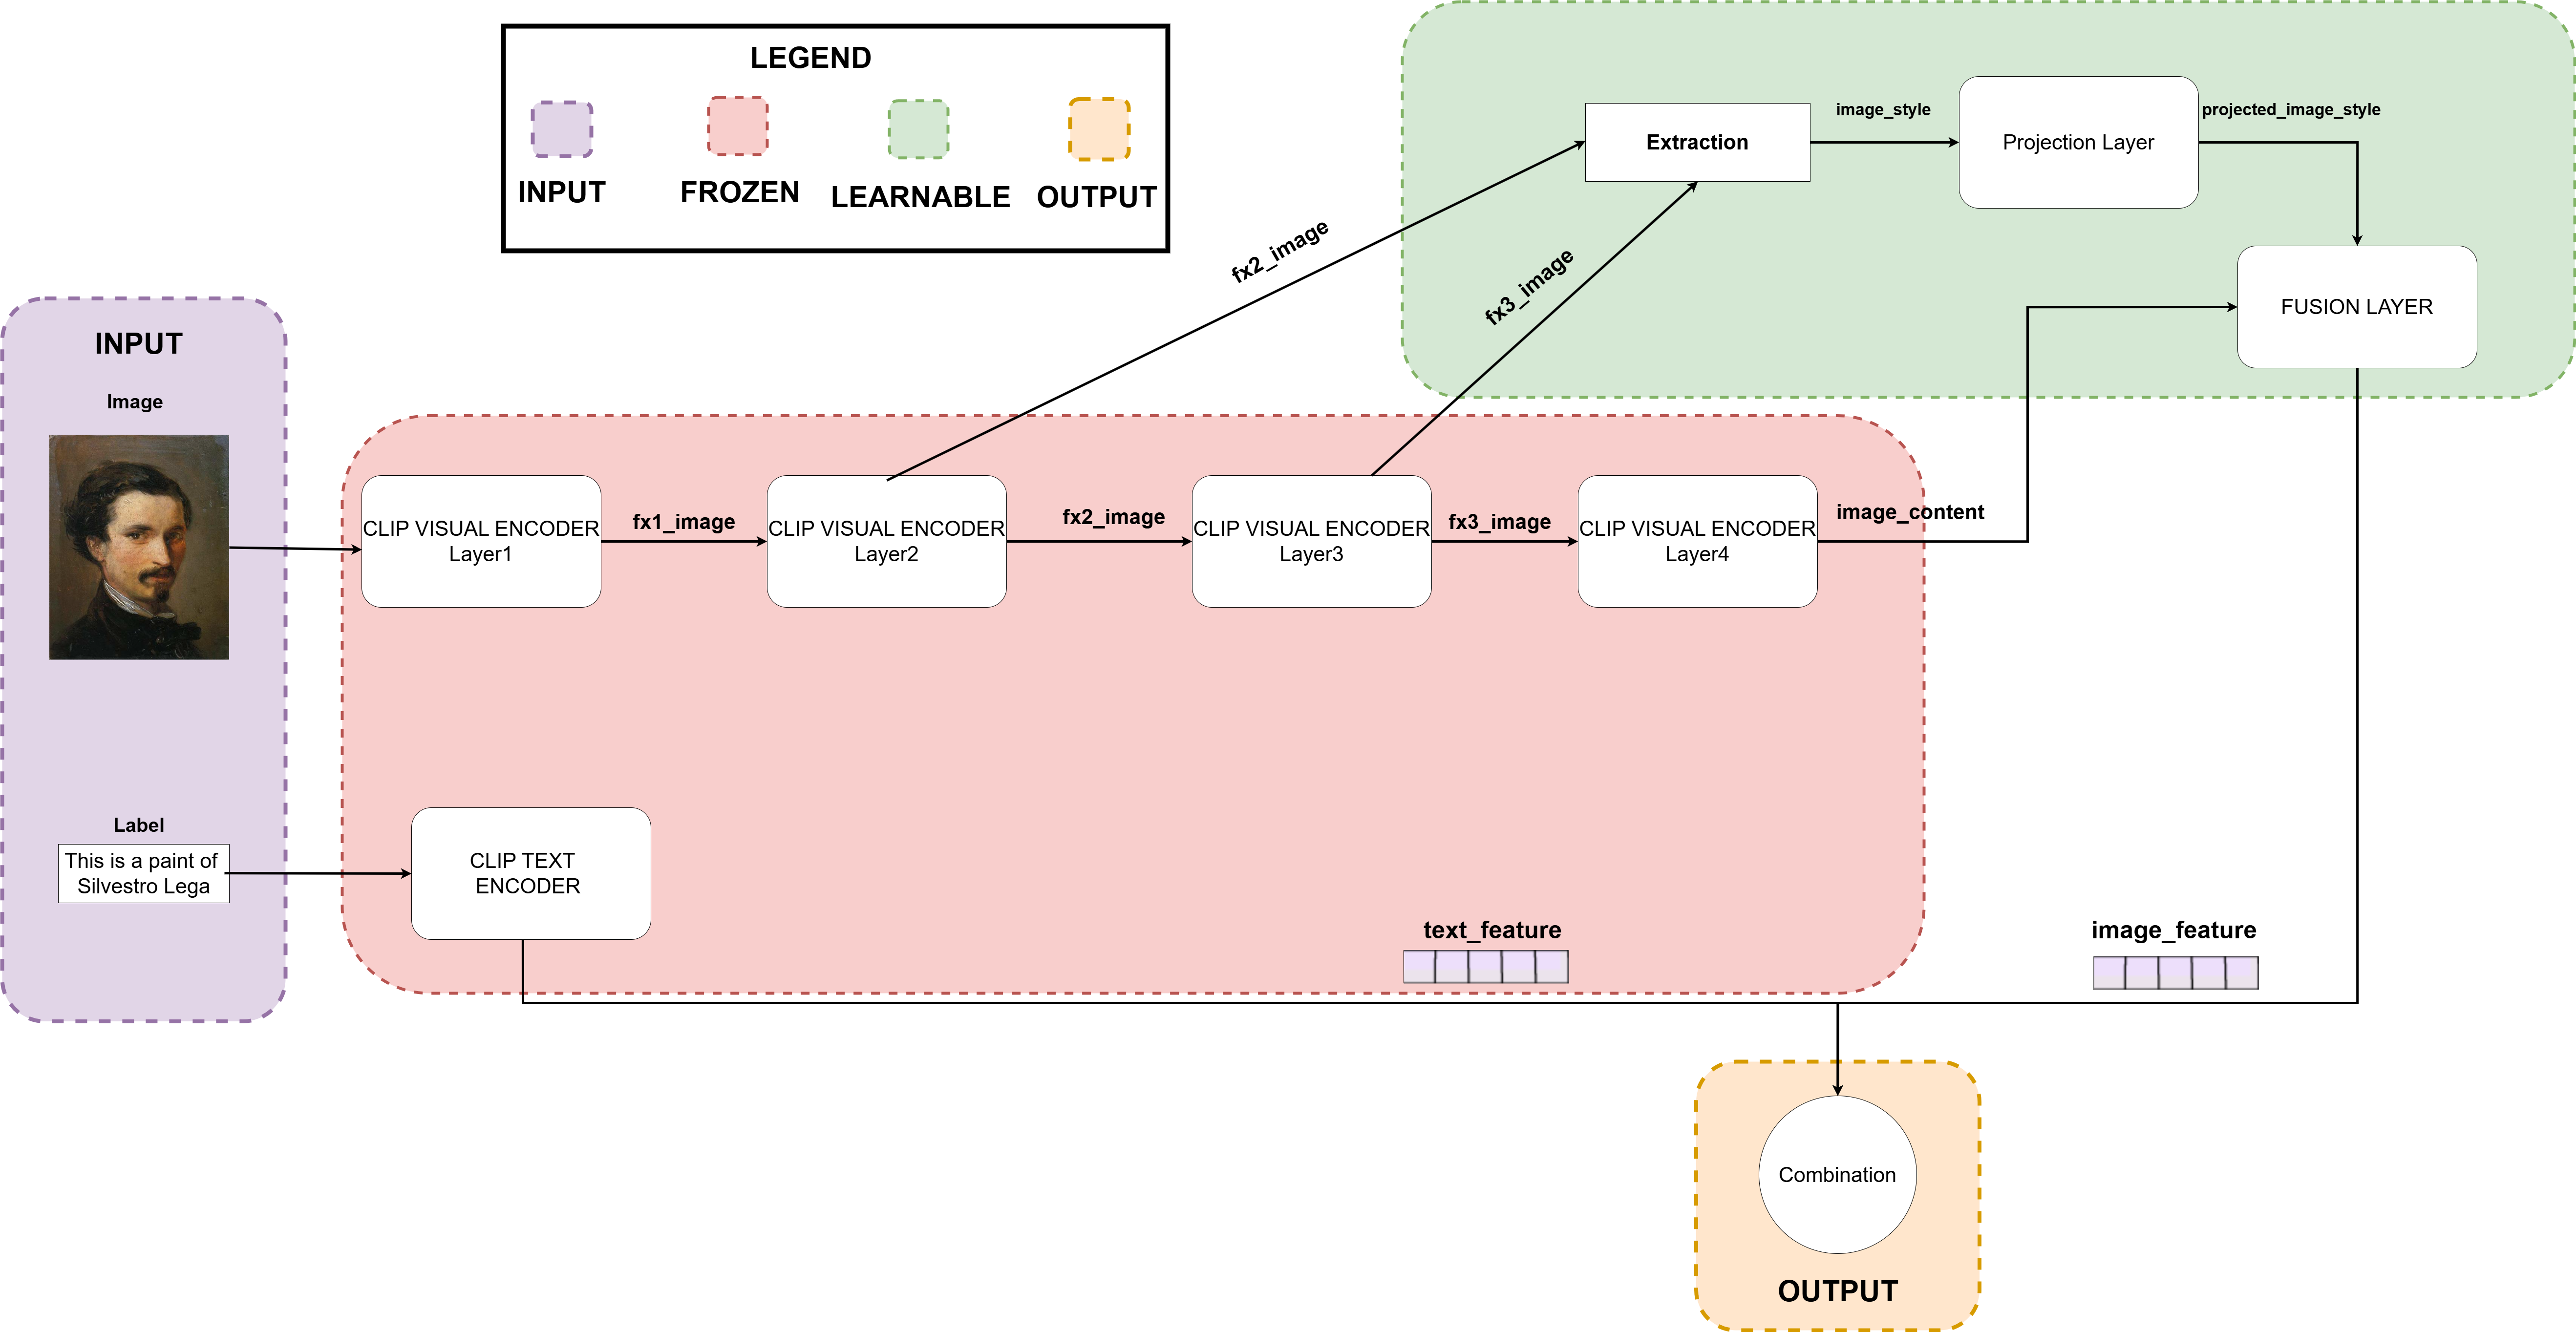
\includegraphics[width=0.9\linewidth,height=0.8\textheight]{../img/StyCLIP.png} % Adjust path if needed
    \caption{StyCLIP Architecture Overview (from paper)}
  \end{figure}
\end{frame}

\begin{frame}
  \frametitle{StyCLIP: Training Strategy}
  \begin{itemize}
    \item \textbf{Frozen Backbone:} Original CLIP (RN50) visual and text encoders are frozen.
    \item \textbf{Trainable Components:} Only the new style projection layers and fusion adapter are optimized.
    \item \textbf{Rationale:}
      \begin{itemize}
        \item Preserve pre-trained semantic knowledge from CLIP.
        \item Reduce computational cost.
        \item Enable efficient fine-tuning on artistic datasets.
      \end{itemize}
  \end{itemize}

  \begin{block}{Hyperparameter Tuning}
    \begin{itemize}
        \item Optuna \cite{Optuna} used for:
        \begin{itemize}
            \item Fusion bottleneck dimension \{64, 128, 256\}
            \item Dropout rate [0.0, 0.5]
            \item Learning rate log-uniform [$10^{-5}, 10^{-3}$]
            \item Weight decay log-uniform [$10^{-6}, 10^{-3}$]
        \end{itemize}
    \end{itemize}
  \end{block}
  \tiny \nocite{Optuna}
\end{frame}

% --- Experimental Setup ---
\section{Experimental Setup}
\begin{frame}
  \frametitle{Experimental Setup}
  \begin{block}{Meta-Learning Training for StyCLIP}
    \begin{itemize}
      \item Prototypical network approach.
      \item Episodic training: N-way (N=10 artists) classification.
      \item K support examples, Q=3 query examples per artist per episode.
      \item Two StyCLIP training configurations:
        \begin{itemize}
          \item \textbf{StyCLIP FLS1}: Trained with K=1 support shot.
          \item \textbf{StyCLIP FLS4}: Trained with K=4 support shots.
        \end{itemize}
    \end{itemize}
  \end{block}

  \begin{block}{Evaluation Protocol}
    \begin{itemize}
      \item N-way classification (all available artists in the test subset).
      \item Tested across K $\in \{1, 2, 4, 8, 16\}$ shots for support set.
      \item \textbf{Statistical Robustness:} 10 different random seeds.
      \item \textbf{Metrics:} Accuracy, Macro-Precision, Macro-Recall, Macro-F1.
    \end{itemize}
  \end{block}
\end{frame}

\begin{frame}
  \frametitle{Baseline Methods \& Backbones}
  \begin{columns}[T]
  \begin{column}{0.5\textwidth}
    \begin{block}{Few-Shot Adaptation Methods}
      \begin{itemize}
        \item CLIP + TIP-Adapter \cite{TipAdapter}
        \item CLIP + APE \cite{APE}
        \item CLIP + GDA-CLIP \cite{GDA_CLIP}
        \item CLIP + TIMO \cite{TIMO}
        \item CLIP + TIMO-S
      \end{itemize}
    \end{block}
  \end{column}
  \begin{column}{0.5\textwidth}
    \begin{block}{Backbones Compared}
      \begin{itemize}
        \item \textbf{CLIP RN50}: Standard CLIP ResNet-50.
        \item \textbf{StyCLIP FLS1}: Our custom backbone, trained with 1-shot.
        \item \textbf{StyCLIP FLS4}: Our custom backbone, trained with 4-shots.
      \end{itemize}
    \end{block}
  \end{column}
  \end{columns}
  An example episode for RN50:
\end{frame}



% --- Results ---
\section{Results}
\begin{frame}
  \frametitle{Hyperparameter Optimization Highlights}
  \begin{columns}[T]
    \begin{column}{0.5\textwidth}
      \begin{block}{StyCLIP FLS1 (1-shot trained)}
        \begin{itemize}
          \item Bottleneck: 64
          \item LR: $6.01 \times 10^{-5}$
          \item Dropout: 0.0
          \item Weight Decay: $4.83 \times 10^{-4}$
          \item Valid Acc: 57.07\%
        \end{itemize}
      \end{block}
    \end{column}
    \begin{column}{0.5\textwidth}
      \begin{block}{StyCLIP FLS4 (4-shot trained)}
        \begin{itemize}
          \item Bottleneck: 128
          \item LR: $1.02 \times 10^{-5}$
          \item Dropout: 0.1
          \item Weight Decay: $1.03 \times 10^{-6}$
          \item Valid Acc: 60.53\%
        \end{itemize}
      \end{block}
    \end{column}
  \end{columns}
\end{frame}



\section{Example Episode for RN50}
\begin{frame}
  \frametitle{Example Episode for RN50}
  \begin{figure}
    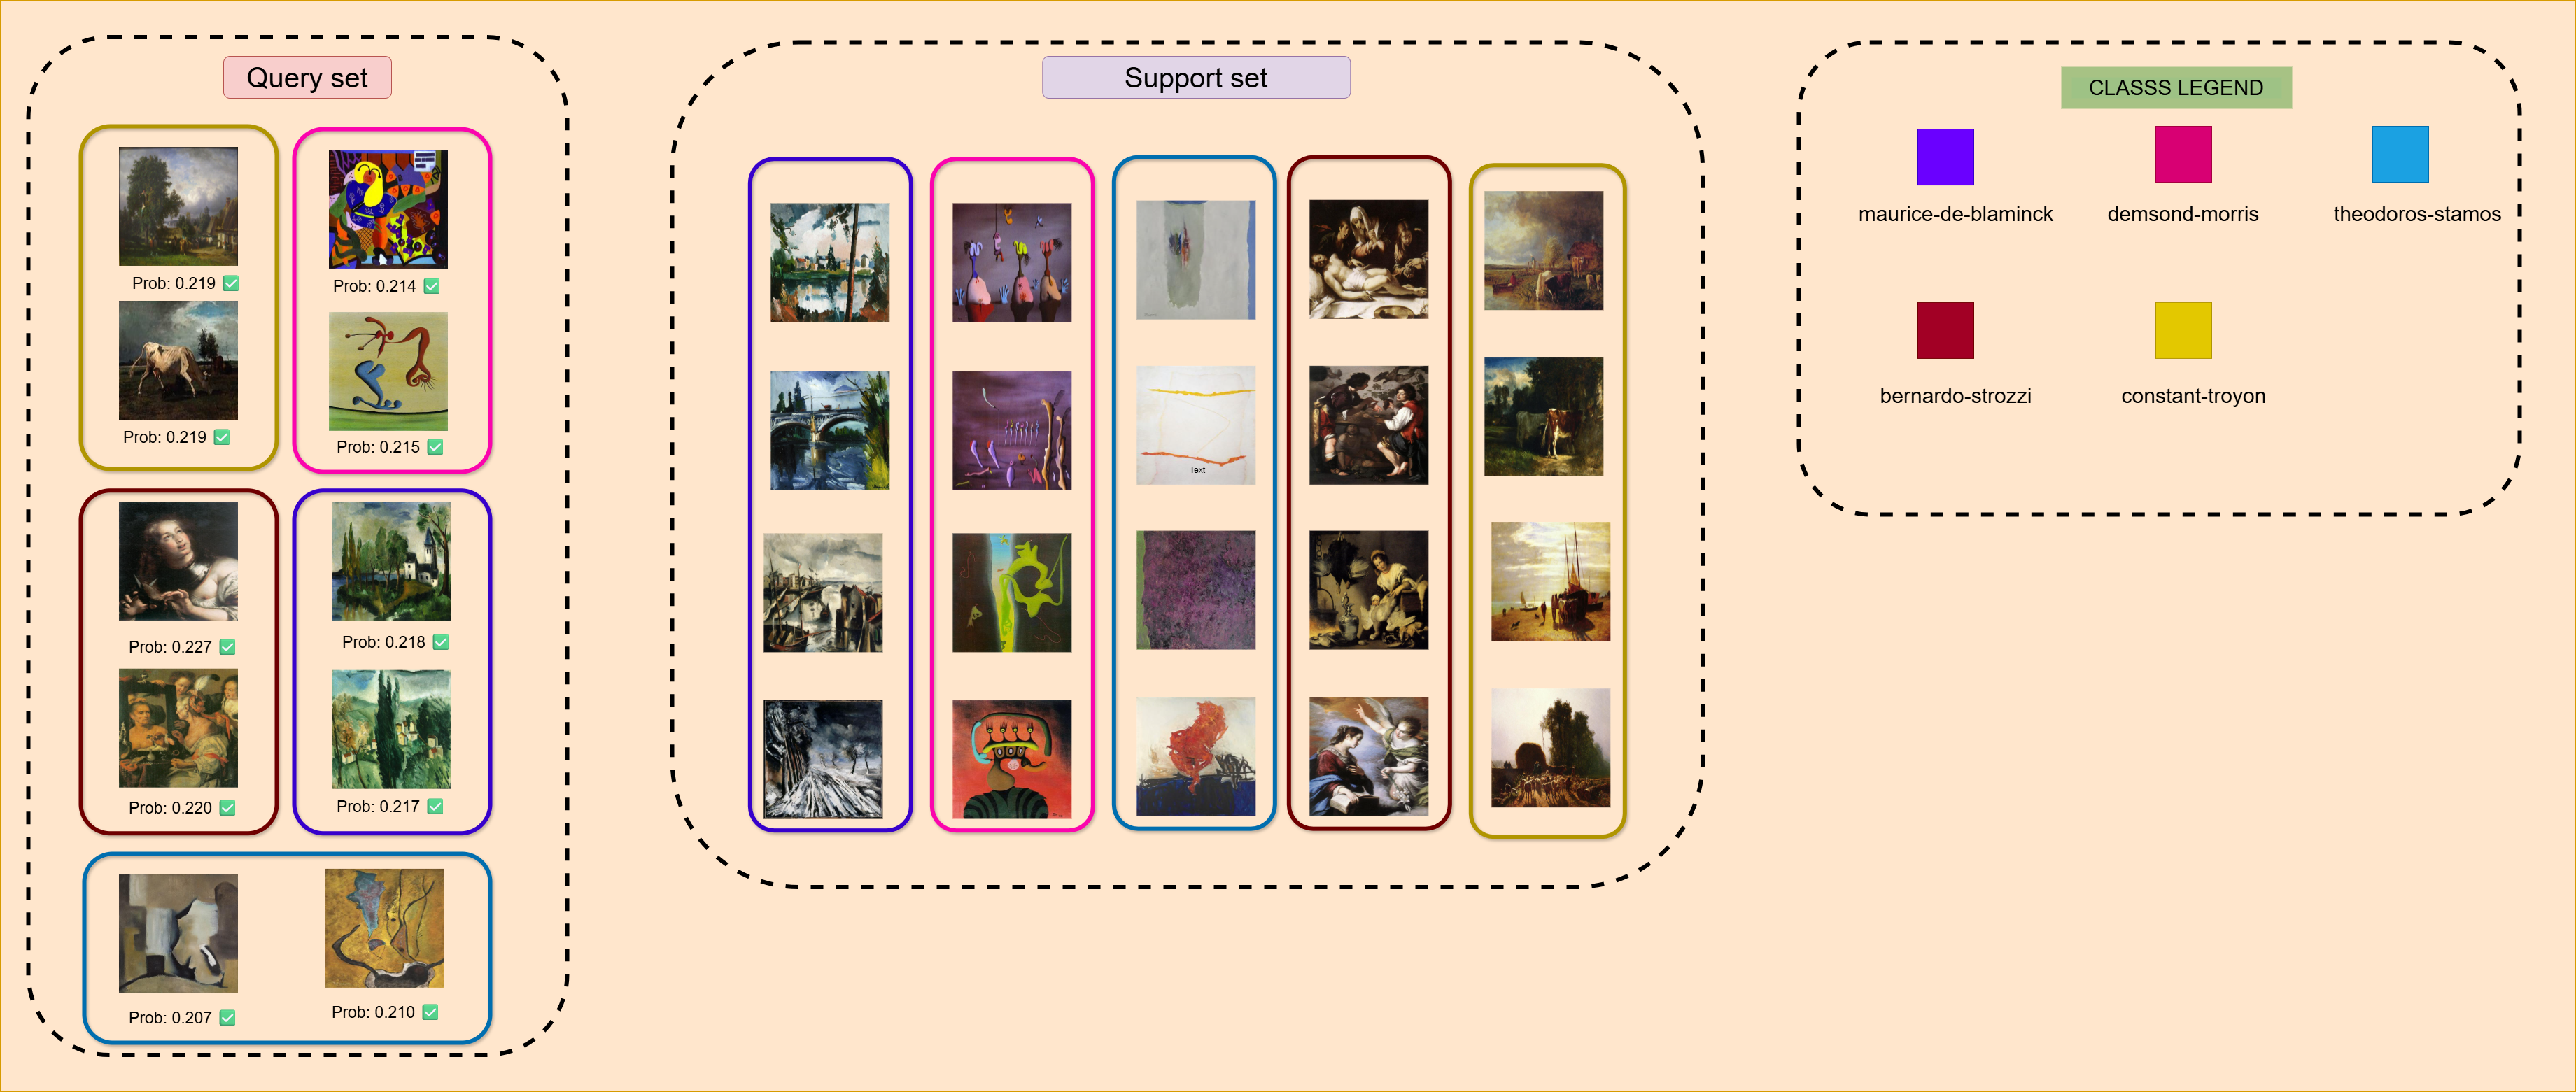
\includegraphics[width=0.8\linewidth]{../img/episode_example.drawio.png} % Adjust path if needed
    \caption{Example episode: 5-Way, 4-Shots ,10 query examples}
  \end{figure}
  \end{frame}



\begin{frame}
  \frametitle{Key Evaluation Results}
  \textbf{Main Finding:} Integrating explicit style-aware features (StyCLIP) \textit{consistently underperforms} standard CLIP variants.

  \begin{itemize}
    \item Standard CLIP with RN50 backbone is the best performing backbone.
    \item StyCLIP backbones (Custom\_FSL1\_RN50, Custom\_FSL4\_RN50) significantly degrade performance for all FSL methods.
    \item TIMO and TIMO-S (our adaptation logic) are the best FSL methods when using the standard RN50 backbone.
  \end{itemize}

  \begin{block}{Example: 16-Shot Classification Accuracy (\%)}
    \centering
    \tiny
    \begin{tabular}{@{}lcc@{}}
      \toprule
      \textbf{Model} & \textbf{Backbone} & \textbf{ACC (\%)} \\
      \midrule
      TIMO           & Custom\_FSL1\_RN50 & 37.00 \\
      TIMO           & Custom\_FSL4\_RN50 & 43.27 \\
      \textbf{TIMO}  & \textbf{RN50}      & \textbf{73.36} \\
      \midrule
      TIMO\_S  & Custom\_FSL1\_RN50 & 39.20 \\
      TIMO\_S  & Custom\_FSL4\_RN50 & 48.75 \\
      \textbf{TIMO\_S } & \textbf{RN50}      & \textbf{73.46} \\
      \bottomrule
    \end{tabular}
    \normalsize
    % \vspace{0.5em} % Removed to save vertical space
  \end{block}
\end{frame}

\begin{frame}
    \frametitle{Statistical Analysis Summary}
    \begin{itemize}
        \item Paired t-tests confirmed the significance of performance differences.
        \item \textbf{Key Observation:} Standard CLIP (RN50) significantly outperforms StyCLIP-trained backbones across nearly all configurations and few-shot methods.
        \item Example: For 16-shot with TIMO\_S:
        \begin{itemize}
            \item RN50 (73.46\%) vs Custom\_FSL4\_RN50 (48.75\%) $\rightarrow$ $\approx$ 25 percentage point difference, statistically significant.
        \end{itemize}
    \end{itemize}
    $\implies$ The architectural changes in StyCLIP for explicit style modeling did not yield benefits and often hindered performance.
\end{frame}


% --- Conclusion ---
\section{Conclusion \& Discussion}
\begin{frame}
  \frametitle{Conclusion \& Discussion}
  \begin{itemize}
    \item \textbf{Main Finding:} Integrating explicit style-aware features via Gram matrices (StyCLIP) did \textbf{not improve} few-shot artist classification performance.
    \item \textbf{Performance:} Standard CLIP (RN50 backbone) consistently outperformed StyCLIP variants.
    \item \textbf{Implication:} Explicit Gram matrix-based style modeling might interfere with CLIP's pre-trained semantic representations rather than enhance them for this task.
    \item \textbf{Future Directions:} Alternative approaches like attention-based style integration or domain-specific fine-tuning (without architectural changes) might be more fruitful.
  \end{itemize}
\end{frame}

% --- Acknowledgments & Code ---
\section{Acknowledgments \& Code}
\begin{frame}
  \frametitle{Acknowledgments}
  \begin{itemize}
    \item This work was proposed by PhD student \textbf{Nicola Fanelli} and \textbf{Prof. Giovanna Castellano} at the University of Bari.
  \end{itemize}
\end{frame}

\begin{frame}
  \frametitle{Code Availability}
  The code for this project is available on GitHub:
  \begin{center}
    \url{https://github.com/Fonty02/ComputerVision/tree/main/TIMO}
  \end{center}
  \vspace{2em}
  \begin{center}
    \Large Thank You!
    \vspace{1em}
  \end{center}
\end{frame}


\begin{frame}[plain, allowframebreaks]
    \frametitle{References}
    \tiny % Make text smaller for references
    \bibliography{bibo}
\end{frame}


\end{document}